%! suppress = LabelConvention
A loop command is a focal construct in many areas of computer science.
In complexity theory\index{complexity theory}, interesting program behavior occurs in loops~\cite{benamram2020,jones2009}.
In verification, loop \emph{invariants}\index{loop invariant} (presented in~\autoref{verification}) are essential for proving program correctness.
However, finding loop invariants is one of the most challenging problems in verification~\cite{dillig2013,si2018,yu2023}.
In compiler theory, loops provide a mechanism for applying \emph{code optimizations}\index{code optimization}.
These are syntactic transformations that aim to improve the efficiency of the generated executable program.
The transformation must preserve semantic equivalence with the original program that contains the loop;
but otherwise, the program structure can be altered to reduce running time, size, power consumption, \etc~\cite[p. 10]{alfred2007}.
In parallel programming\index{parallel programming}, the repetitiveness of loop \emph{iterations} creates potential for executing the iterations in parallel to reduce the program's runtime latency.

This section focuses on automatic compile-time loop \emph{transformations}\index{loop transformation} and relating those transformations to \emph{parallel executions}.
The starting point is a sequential imperative program.
The program result is the one obtained by executing the program's commands in the order they appear;
with appropriate exceptions for control flow constructs like branching and loops.
Thus, the sequential program specifies a precise ordering on the operations that are expected to execute.
It is impossible to exploit parallelism directly from this specification because parallelization changes the operation order.
However, conditional on the \emph{dependence} present in the program,
it may be permissible to allow such an alternative command execution order if it computes the same result as the original sequential program.

\subsubsection{Basic Loop Constructs and Canonicity}
\label{loop-constructs}

Throughout the presentation, we assume a \emph{loop} to mean a \pr|for| loop\footnote{
Extending the presentation to more general loop forms is generally challenging.
Refer to~\autoref{icc-fission} and ~\autoref{sec:vmcai} for an approach that circumvents the limitation.}
in an imperative programming language.
We will refer to~\autoref{lst:loop-ex} to highlight essential concepts and terms.
The examples use the C\index{C} language, but the concepts extend to other imperative languages.
A {loop} has two parts: a header (L\ref{line:header})\index{loop header} and a body (L\ref{line:header-2}--\ref{line:body})\index{loop body}.

\begin{center}
\begin{minipage}{\textwidth}
\captionsetup{type=lstlisting}
\cstarinputlisting[][escapeinside=||]{insertion.c}
\captionof{lstlisting}[Loop of insertion sort]{Adaptation of insertion sort from~\textcite{cormen2009}.}
\label{lst:loop-ex}
\end{minipage}
\end{center}

The \emph{header} contains three expressions that define in order the loop's initialization\index{initialization expression}, update or increment\index{update expression}, and the termination condition\index{termination condition}.
These expressions refer to the loop \emph{iteration variable}\index{iteration variable}, a scalar variable that is updated in each iteration.
At L\ref{line:header}, the iteration variable\index{iteration variable} is \pr|j|.
The iteration variable\index{iteration variable} is initialized, before any iterations occur, by the initialization expression\index{initialization expression}.
The iteration variable\index{iteration variable} is updated after each iteration by the update expression\index{update expression}.
In the initialization expression\index{initialization expression}, the constant \pr|1| is the \emph{lower bound} (lb) of iteration.
In the termination condition\index{termination condition}, \pr|A.length| is the \emph{upper bound} (ub) of iteration~\cite[p. 198--199]{openmp_api}.
In~\autoref{sec:postcond}, when the upper bound is a variable, we call it the \emph{loop guard}\index{guard variable}, or {guard variable}.
The range of iterations is the \emph{iteration space}\index{iteration space}.

The \emph{body}\index{loop body} consists of executable statements~\cite[p. 67]{openmp_api}.
The termination condition\index{termination condition} is evaluated, at each iteration, before executing the commands of the body.
The loop repeats execution of the body until the condition\index{termination condition} evaluates to false.
The body may recursively contain another loop.
Then, the inner loop is called a \emph{nested loop}\index{nested loop}.
In~\autoref{lst:loop-ex}, the header\index{header} of the nested loop is at L\ref{line:header-2} and body\index{loop body} at L\ref{line:body}.
Since there is no intervening code between the two loops, the loop of~\autoref{lst:loop-ex} defines a \emph{perfectly nested loop}\index{perfectly nested loop}~\cite[p. 84]{openmp_api}.

\paragraph*{Canonical loop.}
The canonical loop form simplifies several program analyses and makes transformations more effective~\cite{llvm_loops}.
A \emph{canonical loop}~\cite[p. 196--202]{openmp_api}\index{canonical loop}\footnote{
The definition is specific to the programming model of~\autoref{openmp} and~\autoref{sec:vmcai}.} has form,
\begin{center}
\begin{minipage}{\textwidth}
\captionsetup{type=lstlisting}
\cstarinputlisting{canonical.imp}
\captionof{lstlisting}[Canonical loop form]{Canonical loop form.}
\label{lst:canonical}
\end{minipage}
\end{center}
The header must additionally satisfy the following restrictions\footnote{
Additional restriction are defined in~\cite[p. 201]{openmp_api}.}.
\begin{enumerate}
\item The initialization\index{initialization expression} \pr|init-expr| has form \pr|var=lb| where \pr|var| is the iteration variable and \pr|lb| is the lower bound of iteration.
\item The termination condition\index{termination condition} \pr|test-expr| has form \pr|var op ub| (commutatively)
    where \pr|ub| is the upper bound of iteration and \pr|op| is an operator in \{\pr|<|, \pr|>|, \pr|<=|, \pr|>=|, \pr|!=|\}.
\item The update expression\index{update expression} \pr|incr-expr| applies to \pr|var| an increment or a decrement (\pr|incr|) of 1.
The operation must be in unary (\pr|++|, \pr|--|), compound assignment (\pr|+=|, \pr|-=|), or
binary (\pr|var=var+incr|, \pr|var=incr+var|, \pr|var=var-incr|) form.
\end{enumerate}

\paragraph*{Non-canonical loop.}
If a loop that does not satisfy the criteria of a canonical loop, in~\autoref{sec:vmcai}, it is referred to a \emph{non-canonical loop}\index{non-canonical loop}.

\paragraph*{A note on loop representations.}
This representation is simplified, at least in two ways, for accessibility.
Real compile-time code optimizations are performed
on an \emph{intermediate representation}\index{intermediate representation} (IR) of the source program.
Intermediate representations, which are compiler-specific, differ from the high-level syntactic view described previously.
Further, to facilitate various analyses, it is possible to {detach} programs from language-based representations altogether,
via control-flow (and other) graphs.
A \emph{control-flow graph}\index{control-flow graph} (CFG)~\cite{allen1970} is a directed graph for representing program's execution paths.
In a CFG, the nodes are {basic blocks} and the edges are control flow paths.
A \emph{basic block}\index{basic block} is a linear sequence of program instructions with one entry and one exit point.
Control-flow graphs\index{control-flow graph}
are a common approach for compile-time program analyses and transformations\index{loop transformation}~\cite[p. 48]{moyen2017}
and are adopted, \eg in the LLVM compiler\index{LLVM compiler}~\cite{llvm_loops}.
Although making this note is important, the level of detail is unnecessary for this topic overview.

\subsubsection{Sequential Loop Transformations}
\label{loop-transforms}

Compile-time loop optimization\index{code optimization} is motivated by the idea that a loop {transformation} yields---by some quantifiable metric like data access pattern---a more optimal loop form than the original source program~\cite{alfred2007}.
A loop transformation replaces the \emph{original} loop(s) with one or more semantically equivalent \emph{generated} loops.
We consider next a few common loop transformations to demonstrate the idea.
Assuming a sequential source program, these transformations are straightforward for a compiler to apply automatically~\cite{bertolacci2018}.

\paragraph*{Distributing and combining loops.}
Loop \emph{fusion}\index{loop transformation!fusion}, in~\autoref{lst:fusion}, merges multiple loops by replacing them with a single loop.
In each iteration, the generated loop executes an iteration of each original loop.
Loop \emph{fission}\index{loop transformation!fission}, in~\autoref{lst:fission}, operates in the reverse direction.
It breaks the original loop into multiple loops, with each generated iteration taking only a part of the original loop's body~\cite{zhao2018}.
In both transformations, the loop header and iteration space remain unchanged.

\begin{center}
\begin{minipage}{\textwidth}
\captionsetup{type=lstlisting}
\begin{minipage}{.45\textwidth}
\captionsetup{type=lstlisting}
\cstarinputlisting{fusion.c}
\captionof{lstlisting}[Loop fusion transformation]{Loop fusion.}
\label{lst:fusion}
\end{minipage}\hfill%
\begin{minipage}{.45\textwidth}
\cstarinputlisting{fission.c}
\captionof{lstlisting}[Loop fission transformation]{Loop fission.}
\label{lst:fission}
\end{minipage}
\end{minipage}
\end{center}

\paragraph*{Iteration range-based transformations.}
The \emph{split} transformation\index{loop transformation!split},
in~\autoref{lst:split}, breaks the original loop into multiple generated loops.
Each generated loop has the same body as the original, but iterates over a different contiguous subset of the original range.
Loop \emph{tiling}\index{loop transformation!tile} breaks a loop into contiguous chunks of fixed \emph{tile size}.
In~\autoref{lst:tiling}, the tile size is 8.
Tiling improves cache behavior by reducing data reuse distance~\cite{bertolacci2018}.
Loop \emph{reversal}\index{loop transformation!reversal} executes loop iterations in the reverse order.
For example, if \(0, 1,\ldots, n-2, n-1\) are the logical iteration numbers of a loop, after transformation, the iterations occur in order \(n-1, n-2,\ldots, 1, 0\)~\cite{openmp_api}.

\begin{center}
\begin{minipage}{\textwidth}
\captionsetup{type=lstlisting}
\begin{minipage}{.45\textwidth}
\cstarinputlisting{split.c}
\captionof{lstlisting}[Loop splitting transformation]{Loop splitting.}
\label{lst:split}
\end{minipage}\hfill%
\begin{minipage}{.45\textwidth}
\cstarinputlisting{tiling.c}
\captionof{lstlisting}[Loop tiling transformation]{Loop tiling.}
\label{lst:tiling}
\end{minipage}
\end{minipage}
\end{center}

Finally, loop \emph{peeling}\index{loop transformation!peel}, in~\autoref{lst:peel}, is a special case of loop splitting.
It removes the first few or last iterations from the body and performs them outside the loop.
The loop iteration space is adjusted accordingly.

\begin{center}
\begin{minipage}{\textwidth}
\captionsetup{type=lstlisting}
\begin{minipage}[t]{.45\textwidth}
\cstarinputlisting{peel.c}
\captionof{lstlisting}[Loop peeling transformation]{Loop peeling.}
\label{lst:peel}
\end{minipage}\hfill%
\begin{minipage}[t]{.45\textwidth}
\cstarinputlisting{unroll.c}
\captionof{lstlisting}[Loop unrolling transformation]{Loop unrolling.}
\label{lst:unroll}
\end{minipage}
\end{minipage}
\end{center}

\paragraph*{Modifications of the loop body.}
Loop \emph{unrolling}\index{loop transformation!unroll} expands and duplicates the body commands into similar independent commands.
The update condition is adjusted by an \emph{unroll factor}.
In~\autoref{lst:unroll} the loop body is unrolled twice, therefore the unroll factor is 2\footnote{
The simplified example assumes the transformation does not exceed the array bounds.}.
Unrolling aims to reduce or eliminate evaluations of the loop condition.

\paragraph*{Transforming nested iterations.}

Loop \emph{interchange}\index{loop transformation!interchange} is a transformation on a nested loop.
It changes the loop nesting order by exchanging two iteration variables referenced by a nested loop,
as shown in Listings~\ref{lst:pre-interchange} and~\ref{lst:post-interchange}.

\begin{center}
\begin{minipage}{\textwidth}
\captionsetup{type=lstlisting}
\begin{minipage}[t]{.45\textwidth}
\cstarinputlisting{pre-interchange.c}
\captionof{lstlisting}[Loop before interchange]{Pre-interchange.}
\label{lst:pre-interchange}
\end{minipage}\hfill%
\begin{minipage}[t]{.45\textwidth}
\cstarinputlisting{post-interchange.c}
\captionof{lstlisting}[Loop after interchange]{Post-interchange.}
\label{lst:post-interchange}
\end{minipage}
\end{minipage}
\end{center}

\subsubsection{Dependence in Transformations}
\label{dependence-analysis}

A transformation is permissible if the transformation preserves the semantics of the source program.
Thus, the application of a transformation depend crucially on the execution {relationships} between program statements\footnote{
Compiler literature refers to \emph{statements}, rather than commands and expressions.}.
The source program specifies,  via a series of statements and an ordering of those statements, a set of {execution constraints}.
However, the constraints may be imprecise since not all constraints are needed to preserve the effect of the computation.
For example, in the program fragment \pr|X=42; Y=5;| it is safe to reorder the two statements.
A fundamental challenge in compiler theory concerns determining whether an execution order, that differs from the one specified by the source program,
always computes the same result as the source program.
Dependence is the primary mechanism for determining if code transformation is safe.

A \emph{dependence} is a relation on statements that must be preserved by a transformation~\cite[p. 47]{kennedy2001}.
Informally, for any two statements \pr|S1| and \pr|S2|, if \pr|S1| must be executed before \pr|S2| then \pr|S2| depends on \pr|S1|.
Dependence arises primarily from data access patterns -- if \pr|S2| refers to a value computed by \pr|S1| -- and from conditional branching, when the execution of \pr|S1| decides whether \pr|S2| will execute.
Further, by parametrizing computation over iterations, loops introduce additional special cases of dependence.
A \emph{reordering transformation} is any transformation that changes the code execution order, but does not add or delete statements.
By the fundamental theorem of dependence, a reordering transformation that preserves every dependence in a program preserves the meaning of that program~\cite[p. 66]{kennedy2001}.

\paragraph*{Data and control dependence.}
How data is accessed during computations creates dependencies in terms of \emph{order} of shared memory operations.
There is a \emph{data dependence}\index{data dependence} from statement \pr|S1| to \pr|S2|
if and only if both statements access the same memory location, at least one statement writes to the location,
and there is a runtime execution path from \pr|S1| to \pr|S2|~\cite[p. 59--60]{kennedy2001}.
Dependence is further complicated by the program's control flow.
Conditional branching creates a \emph{control dependence} between the control statement
and the statements whose execution depends on the control statement~\cite[p. 374]{kennedy2001}.
Four common cases of data and control dependence are demonstrated in Listings~\ref{dep-true}--\ref{dep-control}.
The interesting variables, that reference a memory location of interest, are emphasized.

\begin{center}
\begin{minipage}[t]{.4\textwidth}
\captionsetup{type=lstlisting}
\cstarinputlisting[][emph={X},emphstyle={\color{pthread}\textbf},numbers=none,escapeinside={||}]{dep-true.imp}
\captionof{lstlisting}[True dependence]{True dependence.}
\label{dep-true}\index{true dependence}
\end{minipage}\hspace{3em}
\begin{minipage}[t]{.4\textwidth}
\captionsetup{type=lstlisting}
\cstarinputlisting[][emph={X},emphstyle={\color{pthread}\textbf},numbers=none,escapeinside={||}]{dep-anti.imp}
\captionof{lstlisting}[Antidependence]{Antidependence.}
\label{dep-anti}\index{antidependence}
\end{minipage}

\begin{minipage}[t]{.4\textwidth}
\captionsetup{type=lstlisting}
\cstarinputlisting[][emph={X},emphstyle={\color{pthread}\textbf},numbers=none,escapeinside={||}]{dep-out.imp}
\captionof{lstlisting}[Output dependence]{Output dependence.}
\label{dep-out}\index{output dependence}
\end{minipage}\hspace{3em}
\begin{minipage}[t]{.4\textwidth}
\captionsetup{type=lstlisting}
\cstarinputlisting[][emph={X},emphstyle={\color{pthread}\textbf},numbers=none,escapeinside={||}]{dep-control.imp}
\captionof{lstlisting}[Control dependence]{Control dependence.}
\label{dep-control}\index{control dependence}
\end{minipage}
\end{center}

\begin{itemize}
\item A \emph{true dependence}\index{true dependence}\index{dependence!true}
occurs when a write (\pr|S1|) executes before a read (\pr|S2|) at the same memory location (\pr|X|).
True dependence ensures the read observes the value of the write.

\item An \emph{antidependence}\index{antidependence}\index{dependence!anti}
reverses the order,
with a read (\pr|S1|) executing before a write (\pr|S2|) at the same memory location (\pr|X|).

\item An \emph{output dependence}\index{output dependence}\index{dependence!output}
requires two writes  (\pr|S1|, \pr|S2|) to the same memory location (\pr|X|).
It forbids reordering the writes to prevent an interchange that would cause a subsequent read (\pr|S3|) to observe an incorrect value.

\item In \emph{control dependence}, the dependent statement (\pr|S2|) is conditionally executed,
based on evaluation of the control statement (\pr|S1|).
\end{itemize}

\paragraph*{Dependence in loops.}
Data and control dependence are applicable to loops;
however, loops introduce additional dependence.
Dependence in loops arises from statements being \emph{parameterized by iterations} in which they execute.

A \emph{loop-carried dependence}~\cite[p. 73]{kennedy2001}, in~\autoref{lst:loop-carried},
occurs when a statement uses a value computed in a different iteration.
More precisely, a statement \pr|S2| has a loop-carried dependence on statement \pr|S1| if and only if
\begin{enumerate}
\item \pr|S1| references a location \pr|X| on iteration \(i\),
\item \pr|S2| references the location \pr|X| on iteration \(j\), and
\item the loop iterates at least once between the references of \pr|X|, \ie the distance \(d\) between iterations is \(d(i, j) > 0\).
\end{enumerate}

\begin{center}
\captionsetup{type=lstlisting}
\begin{minipage}{.4\textwidth}
\cstarinputlisting[][escapeinside=||]{loop-carried.c}
\end{minipage}%
\hfill%
\begin{minipage}{.5\textwidth}
{\centering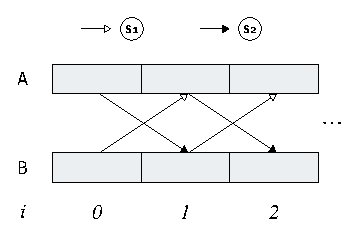
\includegraphics{fig_loop-carry}}
\end{minipage}
\captionof{lstlisting}[Loop-carried dependence]{
Loop-carried dependence.
After the first iteration, in every iteration \pr|S2| uses a value of array \pr|A| computed in the previous iteration by \pr|S1|.
Similarly, \pr|S1| uses a value of array \pr|B| computed in the previous iteration by \pr|S2|.
There is a true dependence from \pr|S2| to \pr|S1| and from \pr|S1| to \pr|S2|, and both dependencies are carried by the loop.
If we select any individual iteration and execute it alone, no dependence exists.
}\label{lst:loop-carried}
\end{center}

If loop statements depend only on statements in the {same iteration}, then there exists a loop-independent dependence.
A \emph{loop-independent dependence}~\cite[p. 76]{kennedy2001} occurs when
\pr|S1| references a location \pr|X| on iteration \(i\),
\pr|S2| references \pr|X| on iteration \(i\),
and there is a control flow path from \pr|S1| to \pr|S2|.

Comparing the two loop dependencies, a loop-carried dependence determines the iteration order and whether that order can be transformed safely.
A loop-independent dependence determines the statement execution order within a nest of loops.

\paragraph*{Dependence analysis.}
Detecting dependencies is the focus of dependence analysis\index{dependence analysis}.
\emph{Dependence analysis} (or a \emph{dependence test})
is a technique for identifying or characterizing program dependencies and dependence-preserving reorderings;
which then may permit transformation or parallel execution.
Among the well-established approaches are
the Banerjee test~\cite{banerjee1997}\index{Banerjee test},
GCD test~\cite{zima199}\index{GCD test},
Omega test~\cite{pugh1991}\index{Omega test},
and commutativity analysis~\cite{rinard1996}\index{commutativity analysis}.
We defer further discussion to~\autoref{sec:vmcai}, that presents a dependence analysis inspired by implicit computational complexity.

\subsubsection{Incorporating Parallelism}

If we only focus on sequential code, the notions around dependence are well-established.
However, sequential reasoning is insufficient for effective use the parallelism that is available in modern processors.
Developing and designing parallel software and algorithms is conceptually challenging.
One of the major difficulties is the effort required to ensure that a parallel program is (functionally) correct.
In addition to all the errors that arise in sequential programs, parallelism introduces a new class of bugs that includes race conditions.
A race condition is devious because the runtime behavior of a program with such a bug is nondeterministic~\cite[p. 32]{chapman2007}.
But in exchange for the challenge, parallelism provides the potential to improve the program's runtime performance.
In practice, exploiting parallelism is necessary for all performance-critical applications~\cite{suomela2022}.

There are several good motivations for introducing parallelism in programs and for improving the existing parallelization techniques.
High-performance multicore processors are ubiquitous and possess the abilities to execute several operations in a single clock cycle.
Due to physics, improvements in hardware design now come from parallel processing capabilities, rather than adjustments in clock cycles.
On the software side, a vast majority of legacy applications, and the algorithms that power them, were developed without parallelization in mind.
\emph{Parallelizing compilers}, that automatically translate sequential programs to multicore executables, have made big advances toward improving prevalence of parallelism.
But despite the advances, these compilers make conservative choices and miss opportunities to parallelize~\cite{holewinski2012}.
Correct and efficient parallel code is thus often hand-crafted in a process that is time-consuming and error-prone.

Ultimately, our abilities to parallelize programs relies on the potential parallelism available in the program and the processor;
and the degree to which we can extract parallelism from a sequential program and find the best parallel schedule under the processor's scheduling constraints~\cite{alfred2007}.
No parallelization strategy fits all cases and it is important to facilitate the discovery of new strategies and parallel algorithms as complementary to existing techniques.
For example, running automatic analysis on a large application can distinguish regions that can be parallelized automatically from those that need manual changes.

\paragraph*{From dependence to independence.}
Since dependence determines how program executions may be reordered, it provides a strong foundation for developing techniques to increase the parallelism available in programs.
Parallelism inherently requires \emph{independence} between statements;
in other words, we are interested in absence of dependence.
Thus, if we can design algorithms, or transform programs in ways that increase prevalence of independent statements, we improve the program's parallelization potential.
One focus area in parallelization concerns \emph{loop-level parallelism} that aims is to extract parallel tasks from loops.
For example, by the Loop Parallelization Theorem, it is permissible to convert a sequential loop to a parallel one if the loop carries no dependence~\cite[p. 82]{kennedy2001}.
The remainder of this section focuses precisely on the terms and techniques of parallelizing loops.

\paragraph*{Parallel programming models.}
Multiple sophisticated programming models exist to simplify the task of writing parallel programs.
These models raise the abstraction level between the application code and the operating system-level parallelization mechanism of threading.
The OpenMP\index{OpenMP}\index{parallel programming model!OpenMP}
application programming interface is presented in~\autoref{openmp}.
Other approaches include the
\emph{Parallel Patterns Library} (PPL)\index{PPL}\index{parallel programming model!PPL}~\cite{ppl2021,campbell2011},
that parallelizes tasks through built-in algorithms and containerization;
and the \emph{oneAPI Threading Building Blocks} (oneTBB)\index{oneTBB}\index{parallel programming model!oneTBB},
a runtime-based model for \pr|C++|\index{C++} programs~\cite{onetbb}.

\subsubsection{The OpenMP Programming Model}
\label{openmp}

{OpenMP}\index{OpenMP}\index{parallel programming model!OpenMP}, for Open Multi-Processing,
is a parallel programming model for developing portable, shared memory\index{shared memory} parallel applications in
\pr|C|\index{C},
\pr|C++|\index{C++} and
\pr|Fortran|\index{Fortran}~\cite{openmp_api}.
OpenMP is not a programming language;
rather, it provides directives for sequential programs that translate the programs to parallel execution instructions at compile-time.
The OpenMP\index{OpenMP} infrastructure includes compiler directives, library routines, environment variables, and tool support for creating, debugging, and analyzing parallel applications.

Program execution in OpenMP follows the \emph{fork-join programming model}~\cite[p. 24]{chapman2007}\index{fork-join programming model} of~\autoref{fig:fork-join}.
Program execution starts with an {primary thread}\index{primary thread}
%\footnote{Color \tikz\draw[pthread,fill=pthread] (0,0) circle (.5ex); is the primary thread in drawings.}
that runs in sequential mode.
After encountering a specially-marked parallelizable program region, the primary thread spawns a team of threads in a \emph{fork}\index{fork}-operation.
The team collaborates to complete the tasks of the parallel program region.
The execution concludes with a \emph{join}\index{join}-operation, where the forked threads terminate.
The primary thread\index{primary thread} continues execution past the parallel program region\index{parallel region}, running again in sequential mode.

\begin{figure}[H]
\centering
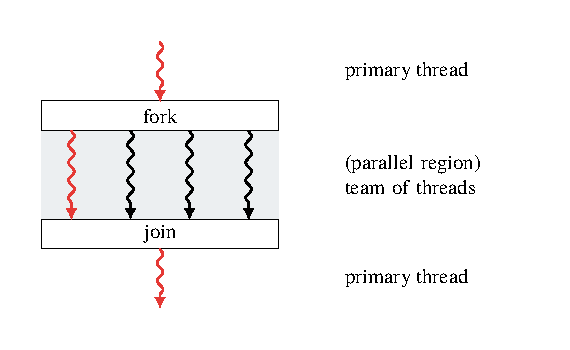
\includegraphics{fig_fork-join}
\caption[The fork-join programming model]{The fork-join programming model.}
\label{fig:fork-join}
\end{figure}

In OpenMP, a programmer annotates {structured blocks} with parallelization {directives} to control the parallel execution behavior.
A \emph{structured block}\index{structured block} is a block of executable statements with a single point of entry and exit.
A \emph{parallelization directive}\index{parallelization directive} is a syntactical comment that specifies instructions for how the {structured block}\index{structured block} should be executed.
The syntax and semantics of {parallelization directives}\index{parallelization directive} are defined by OpenMP\index{OpenMP}.
It the responsibility of the programmer to apply the directives safely.
During compilation, an OpenMP\index{OpenMP}-aware compiler translates the directives into parallel-executable instructions~\cite{oak-slides}.
Other compilers a free to ignore the directives.
OpenMP\index{OpenMP} applications are suitable for running on multicore chips, GPUs\index{GPU}, and various other devices attached to a CPU\index{CPU}.
OpenMP is developed and maintained by the OpenMP Architecture Review Board (ARB).

\paragraph*{Foundational terms.}
The following are basic parallel programming terms needed to discuss OpenMP directives~\cite{openmp_api};
refer to \autoref{lst:parallel} for a visual.
A \emph{thread}\index{thread} is a logical {execution entity}, equipped with a stack and associated thread-specific memory.
The threads are identified by numeric ids.
Once a non-empty set of threads is assigned to execute implicit tasks of a parallel region, the {set of threads} becomes a \emph{team}\index{team}.
\emph{Region}\index{region} refers to all {code} encountered during execution, including code encountered in called procedures.
A region is a \emph{parallel region}, if it has an associated set of implicit tasks, and has been assigned a team to execute those tasks.
A \emph{task}\index{task} is a specific instance of {executable code and its data environment} that can be scheduled for execution.
If a task is generated by an implicit parallel region, or through an encounter with a parallel construct during execution, it is an \emph{implicit task}.
Finally, a \emph{barrier}\index{barrier} is a blocking synchronization construct at a program {execution point}.
No thread in a team may execute beyond a barrier until all team members have reached the barrier.

Additional terminology relates to parallelization of loops.
A \emph{worksharing loop}\index{worksharing loop} is a loop-associated construct that satisfies
the worksharing loop property\index{worksharing loop property}.
The \emph{worksharing loop property}\index{worksharing loop property} requires that a construct
distributes the iterations of the associated loops among the threads\index{thread} of the team that encounters the loop~\cite[p. 113]{openmp_api}.

\paragraph*{Essential parallel directives.}
{Parallelization directives}~\index{parallelization directive} are at the core of OpenMP\index{OpenMP}.
This section introduces a few important ones, including the directives that appear elsewhere in this dissertation.
Because OpenMP is a powerful and rich programming model, it is possible to present only a light introduction.
A complete definition is available in the OpenMP API technical specification~\cite{openmp_api}.

\begin{itemize}

\item \texttt{\#}\omp{pragma omp}
is a directive specification in the style of
\pr|C|\index{C}/%
\pr|C++|\index{C++}.
A {parallelization directive}~\index{parallelization directive} must start with these keywords.

\item The \omp{parallel} construct
marks a {structured block}~\index{structured block} parallelizable~\cite[p. 384--385]{openmp_api}.
\autoref{lst:parallel} shows the syntactic use and illustrates its behavior.
When a thread\index{thread} encounters the \pr|parallel| construct,
it forms a {team of threads} to execute the associated {structured block}\index{structured block}.
The structured block becomes a {parallel region}\index{parallel region}.
The thread that encountered the \pr|parallel| construct is the \emph{primary thread}\index{primary thread} of the team.
All threads in the team execute the {parallel region}\index{parallel region}.
An implicit \emph{barrier}\index{barrier} occurs at the end of a {parallel region}\index{parallel region}.
After the parallel region, the {primary thread}\index{primary thread} resumes execution of the enclosing region.

\end{itemize}

\begin{center}
\captionsetup{type=lstlisting}
\begin{minipage}{.45\textwidth}
\ompcodeinputlisting{parallel.c}
\end{minipage}\hfill%
\begin{minipage}{.5\textwidth}
\hfill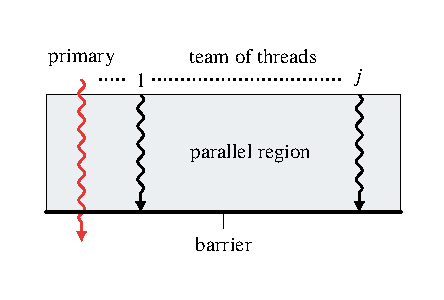
\includegraphics{fig_openmp}
\end{minipage}
\captionof{lstlisting}[The OpenMP \texttt{parallel} construct]{
The OpenMP \pr|parallel| construct and parallel execution with \(j\) threads.%
\index{barrier}\index{thread}\index{parallel region}
}\label{lst:parallel}
\end{center}

\paragraph*{Synchronization constructs.}
Synchronization constructs~\cite[p. 473--482]{openmp_api} enable controlling co-operation of threads\index{thread} over parallel executions.

\begin{itemize}

\item The \omp{atomic} construct ensures a specific memory location is accessed atomically.
It ensures that possible simultaneous reads and writes by multiple threads\index{thread} do not result in indeterminate values.

\item The \omp{barrier} construct specifies an explicit synchronization barrier\index{barrier}.
It prevents any thread\index{thread} from continuing past the barrier until all threads of the sane team encounter the barrier.

\item The \omp{critical} construct means execution of a structured block is restricted to a single thread\index{thread} at a time.

\item The \omp{nowait} clause overrides any synchronization that would otherwise occur at the end of a structured block.
Thus, \omp{nowait} enables specifying that an implicit barrier should not occur.

\end{itemize}

\begin{center}
\begin{minipage}{\textwidth}
One thread\index{thread} executes each iteration sequentially, \(\text{total time} = N \times t_\text{iter}\).
\begin{center}
\captionsetup{type=lstlisting}
\begin{minipage}{.45\textwidth}
\cinputlisting{serial-exec.c}
\end{minipage}\hfill%
\begin{minipage}{.45\textwidth}
\hfill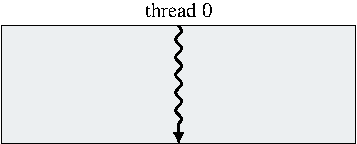
\includegraphics{fig_exec-seq}
\end{minipage}
\captionof{lstlisting}[Serial execution]{Serial execution.}
\label{lst:serial}
\end{center}
All available threads\index{thread} will execute each iteration sequentially, overwriting values of array \pr|C|, \(\text{total time} = N \times t_\text{iter}\).
\begin{center}
\captionsetup{type=lstlisting}
\begin{minipage}{.45\textwidth}
\ompcodeinputlisting{parallel-loop.c}
\end{minipage}\hfill%
\begin{minipage}{.45\textwidth}
\hfill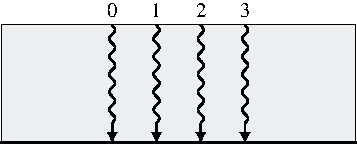
\includegraphics{fig_exec-parallel}
\end{minipage}
\captionof{lstlisting}[Parallel execution]{Parallel execution.\ompi{parallel}\ompi{pragma omp}}
\label{lst:just-parallel}
\end{center}
Assuming a thread\index{thread} count of 4, the threads distribute the loop iteration space uniformly, \(\text{total time} = \frac{N}{4} \times t_\text{iter}\).
\begin{center}
\captionsetup{type=lstlisting}
\begin{minipage}{.45\textwidth}
\ompcodeinputlisting{parallel-for.c}
\end{minipage}\hfill
\begin{minipage}{.45\textwidth}
\hfill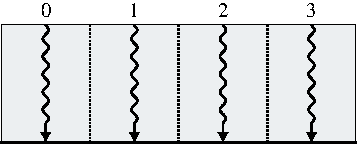
\includegraphics{fig_exec-for}
\end{minipage}
\captionof{lstlisting}[Parallel worksharing]{Parallel worksharing.\ompi{for}\ompi{parallel}\ompi{pragma omp}}
\label{lst:parallel-for}
\end{center}
\captionof{figure}[Parallel worksharing in loop executions]
{The impact of applying parallel worksharing directives to loop executions, adapted from~\textcite{oak-slides}.}
\label{fig:parallel-for}
\end{minipage}
\end{center}

\paragraph*{Work distribution and tasking constructs.}
Parallel executions of structured blocks are controllable by work distribution and tasking directives.
Looping operations on arrays and matrices, like images and tabular data, are often prime candidates for parallelization.
OpenMP has specialized directives to support parallelization of loops.
When applying parallelization directives, the programmer must make sure that the loop is safe to parallelize and performs a sufficient amount of work to benefit from parallelization.

\begin{itemize}

\item The \omp{for} construct is a worksharing loop\index{worksharing loop}.
It specifies that the iterations of associated loop(s) will execute in parallel~\cite[p. 416]{openmp_api}.
The team\index{team} that encounters the loop will perform its execution.
The sequential iteration order is consistent with the execution of the collapsed iterations of a parallel \omp{for} region\index{parallel region}.
The \omp{for} construct supports \eg explicit scheduling, and is compatible with the \omp{nowait} clause.
The \omp{schedule} clause specifies how the loop iterations are divided into chunks and how the chunks are distributed between threads.
The basic use and effect of the \omp{for} construct are demonstrated in~\autoref{fig:parallel-for} and in ~\autoref{lst:parallel-for}.

\item The \omp{loop} construct
supports compiler optimization and parallelization of loops for which logical iterations may execute in any order, including concurrently~\cite[p. 423--424]{openmp_api}.
More precisely, it specifies that the iterations of the associated loop(s) may execute concurrently, in the order specified by an \omp{order} clause.
A loop construct is a worksharing construct if and only if its binding region is the innermost enclosing \omp{parallel} region\index{parallel region}.
It is possible to use a shortcut expression \omp{parallel loop}, combining the two constructs, if the construct refers to one or more loops and no other statements.

\item The \omp{single} construct restricts the execution of a structured to one thread\index{thread}~\cite[p. 405]{openmp_api}.
The executing thread is not necessarily the primary thread;
the choice is implementation-specific.
An implicit barrier\index{barrier} concludes a \omp{single} region.

\end{itemize}

\paragraph*{Shared vs. private data.}
In a multi-threaded shared memory environment, it is necessary to specify how variables are accessed by the executing threads\index{thread}.
This behavior can be controlled with the data-sharing attribute clauses~\cite[p. 224--225]{openmp_api} that are a kind of data environment modifiers.
Both clauses presented here take as a parameter a list of variables names or procedure pointers.
The use of data-sharing attribute clauses is demonstrated in~\autoref{lst:para-block}.

\begin{itemize}

\item The \omp{private} clause privatizes the variables in the parameter list.
It creates a new variable for each variable in the parameter list, and for each thread\index{thread} executing the parallel region\index{parallel region}.
Thus, each thread has its a thread-specific variable copy.
A private variable is uninitialized.

\item The \omp{shared} clause declares that the variables appearing in the parameter list will be shared across the threads\index{thread} executing the parallel region.
The programmer must ensure, with proper synchronization, that the shared memory remains available until execution of the parallel region\index{parallel region} completes.

\end{itemize}

\begin{example}[Parallel transformation]\label{ex:seq-transformation}

We demonstrate a parallelization transformation inspired by~\textcite{singal2019}.
The original sequential code is in~\autoref{lst:seq-block}, where a loop iterates over
fixed-size array length \pr|N|, manipulating each array index in arrays \pr|A| and \pr|B|
(we assume both arrays to be of length \pr|N|).

\begin{center}
\begin{minipage}{\textwidth}
\begin{minipage}{.45\textwidth}
\captionsetup{type=lstlisting}
\cinputlisting{seq-block.c}
\captionof{lstlisting}[Sequential version]{Sequential version.}
\label{lst:seq-block}
\end{minipage}\hfill%
\begin{minipage}{.45\textwidth}
\ompcodeinputlisting{para-block.c}
\captionof{lstlisting}[Parallel version]{Parallel version.\ompi{private}\ompi{shared}\ompi{for}\ompi{parallel}\ompi{pragma omp}}
\label{lst:para-block}
\end{minipage}
\end{minipage}
\end{center}

In~\autoref{lst:para-block}, the loop iteration space is distributed equally between the threads of a team.
Given a team of \(j\) threads, each thread will roughly complete the work of \(N/j\) iterations.
OpenMP often makes the parallelization step straightforward, in this case requiring just one line of directives.
By the data-sharing attribute clauses, the arrays \pr|A| and \pr|B| are explicitly shared across
the threads\index{thread} and the iteration variable \pr|i| is privatized.
\end{example}

\subsubsection{Built-In Loop Transformations in OpenMP}
\label{openmp-transforms}

OpenMP includes built-in directives that perform loop transformations\index{loop transformation}~\cite{openmp_api}.
A loop-transformation replaces the associated loop with a structured block\index{structured block}
that is another loop or a loop sequence.
Unless otherwise specified, all generated loops have canonical form\index{canonical loop}.
Loop-iteration variables of generated loops are always \omp{private} in the innermost enclosing construct.
The loop transformations available in OpenMP are:
fusion\index{loop transformation!fusion},
interchange\index{loop transformation!interchange},
reverse\index{loop transformation!reversal},
split\index{loop transformation!split},
stripe\index{loop transformation!stripe} (interleaving of loop iterations),
tile\index{loop transformation!tile}, and
unroll\index{loop transformation!unroll}.
As an example, we consider the unrolling transformation.

\paragraph*{Loop unrolling.}\index{loop transformation!unroll}
The \omp{unroll} clause~\cite[p. 381--382]{openmp_api}
transforms the associated loop based on the specification provided in the parallelization directive\index{parallelization directive}.
The \omp{unroll} clause is followed by either \omp{full} or \omp{partial} clause.
The effect of \omp{full} clause is to unroll the associated loop fully.
Full unroll requires that the iteration count of the associated loop is a constant.
\autoref{lst:full-unroll} shows the application of the directive and the loop post-transformation form is shown in~\autoref{lst:post-full-unroll}.

\begin{center}
\begin{minipage}{\textwidth}
\captionsetup{type=lstlisting}
\begin{minipage}{.45\textwidth}
\ompcodeinputlisting{full-unroll.c}
\captionof{lstlisting}[Applying full unroll]{Applying full unroll.}
\label{lst:full-unroll}
\end{minipage}\hfill%
\begin{minipage}{.45\textwidth}
\cinputlisting{full-unroll-post.c}
\captionof{lstlisting}[Fully transformed loop]{Fully transformed loop.}
\label{lst:post-full-unroll}
\end{minipage}
\end{minipage}
\end{center}

The \omp{partial} clause takes an integer-valued \emph{unroll factor}\index{unroll factor}.
The effect of \omp{partial} clause is to tile the loop, using the unroll factor as the tile size.
Then, the generated tile\index{loop transformation!tile} loop is fully unrolled.
If no unroll factor\index{unroll factor} is specified, the unroll behavior depends on the implementation.
Partial transformation is illustrated in \autoref{lst:pt-unroll} and~\autoref{lst:post-pt-unroll}.

\begin{center}
\begin{minipage}{\textwidth}
\captionsetup{type=lstlisting}
\begin{minipage}{.45\textwidth}
\ompcodeinputlisting{pt-unroll.c}
\captionof{lstlisting}[Applying partial unroll]{Applying partial unroll.}
\label{lst:pt-unroll}
\end{minipage}\hfill%
\begin{minipage}{.45\textwidth}
\cinputlisting{pt-unroll-post.c}
\captionof{lstlisting}[Partially transformed loop]{Partially transformed loop.}
\label{lst:post-pt-unroll}
\end{minipage}
\end{minipage}
\end{center}

Applying loop transformations\index{loop transformation} requires suitable loop form.
For example, the worksharing loop expects loops to be in canonical form\index{canonical loop}.
Afterward, a transformation that increases the program's parallelization potential\index{parallelization potential} enables making use of multicore hardware during execution.
Thus, an important challenge of parallelizing compilers and program optimizations is to find generalized strategies to increase parallelization potential.

\subsubsection{ICC for Parallel Loop Transformations}
\label{icc-fission}

Since implicit computational complexity has developed many systems for reasoning about loops, it seems natural that in extended use, it has potential to support loop-based program transformations.
Founded on this concept,~\autoref{sec:vmcai} presents an ICC-based technique to increase parallelization potential in imperative programs.
The technique uses a static data dependence analysis that detects independent blocks of commands inside loops.
Through a loop fission\index{loop transformation!fission} transformation,
then independent blocks are then transformed into multiple parallelizable loops, as illustrated in~\autoref{fig:icc-fission}.

\begin{figure}[h]
{\centering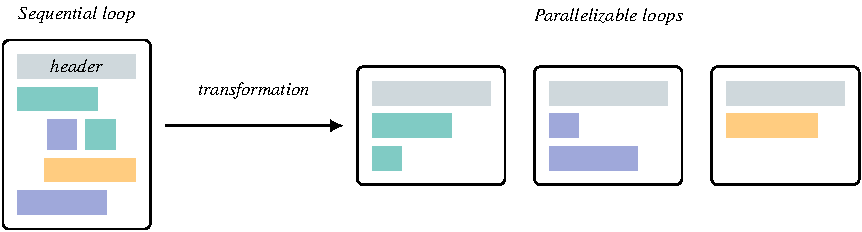
\includegraphics[width=\textwidth,keepaspectratio]{fig_parallel}}
\caption[Loop fission transformation]
{Loop fission of a sequential loop into parallelizable loops.
The loop header (the leading \langclr{header} block) is replicated across the generated loops.
Each generated loop takes a part of the original loop's body.}\label{fig:icc-fission}
\end{figure}

The technique is interesting because it is applicable even when the loop iteration space is unknown;
enabling parallelization of \eg \pr|while| loops.
Such non-canonical loops are traditionally outside the built-in transformation and parallelization capabilities of parallel programming models like OpenMP\@.
Although the \emph{iterations} of \pr|while| loops must be executed under the \omp{single} construct,
the \emph{multiple loops} generated by the transformation can be parallelized with OpenMP directives.
The technique is useful as a preprocessor, before adding parallelization directives;
and in conjunction with other loop transformations.
The technique is inspired by~\cite{moyen20172}, but was adjusted significantly to support the different application.
